\documentclass[border = 5mm]{standalone}
%\documentclass[dvisvgm]{minimal}

\usepackage{tkz-euclide}

\usepackage[OT1]{fontenc}
\usepackage{sansmathfonts}

\begin{document}
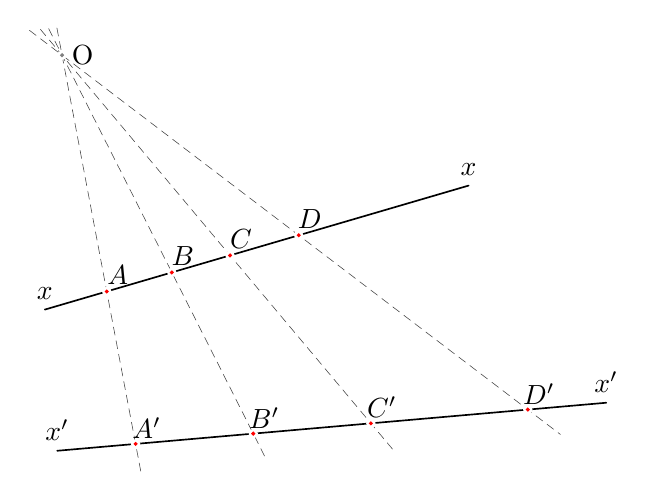
\begin{tikzpicture}[rotate=5]

% Draw line x' with A', B', C', and D'
\tkzDefPoints{0/0/A', 1.5/0/B', 3/0/C', 5/0/D'}
\tkzDrawLines[add = 0.2 and 0.2, semithick](A',D')

% Point O
\tkzDefPoint(-0.5,5){O}

% Draw line x 
\tkzDefPoints{0/2/X, 5/3/Y}
\tkzDrawLine[add = 0.2 and -0.1, semithick](X,Y)

% Projection lines
\tkzDrawLines[gray!150, add = 0.07 and 0.07, densely dashed, very thin](O,A' O,B' O,C' O,D')

% Intersections of projection lines with x
\foreach \i\j in {A'/A, B'/B, C'/C, D'/D} {
\tkzInterLL(O,\i)(X,Y) \tkzGetPoint{\j}
}

\tkzDrawPoints[color=white, size=3](A,B,C,D,A',B',C',D',O)
\tkzDrawPoints[color=red, size=1](A,B,C,D,A',B',C',D') 
\tkzDrawPoints[color=gray, size=1](O)   

% Label points and lines
\tkzLabelPoints[xshift=4, yshift=13](A,B,C,D,A',B',C',D') {A,B,C,D,A',B',C',D'}
\tkzLabelPoint[right](O){O} 
\tkzLabelLine[pos=-0.2, above=0.1pt](X,Y){$x$}  
\tkzLabelLine[pos=0.9, above=0.1pt](X,Y){$x$}
\tkzLabelLine[pos=-0.2, above=0.1pt](A',D'){$x'$}     
\tkzLabelLine[pos=1.2, above=0.1pt](A',D'){$x'$}

\end{tikzpicture}
\end{document}
